\chapter{System Architecture}
\label{chp:architecture} 

\noindent The purpose of this thesis is to build an end-to-end system, that will be able to transfer data all the way from a \gls{microcontroller} to a server. This chapter will describe in detail how the different components of the testbit are connected, and how the different protocols have been configured to read, process and transfer data efficiently. 

\begin{figure}[ht]
    \centering
    \includegraphics[width=0.89\textwidth]{architectureIntro4.png}    
    \caption{End-to-End architecture in the presented system}
    \label{fig:systemArchitectureThisSystem}
\end{figure}


\noindent Figure \ref{fig:systemArchitectureThisSystem} shows how the complete end-to-end system of this thesis is set up. In short terms, the \gls{ADXL345} is connected to the \gls{nRF52}, using the \gls{i2c} interface. The \gls{nRF52} is connected to a  \gls{Raspberry Pi} using \gls{6lowpan} and \gls{ble}. The \gls{Raspberry Pi} is connected to the \gls{lan}, and can therefore forward data to a central stationary computer if additional computational power is needed. Otherwise the results can be sent to the web, to a screen or anywhere else. Several \glspl{microcontroller} can possibly be connected to a Pi at the time, forming a star network. Up to eight connections have been tested successfully in this network. 
 
\noindent There are three main limitations in a system as this:

\begin{itemize}
  \item Computational power in the different nodes
  \item Battery capacity of the end nodes
  \item Network limitations between the nodes
\end{itemize}

%Computations can now either be done in the end nodes at the \textit{nRF52s}, at the \textit{Raspberry Pi}, or forwarded to a web server or another computer with more computational power. Data can also be displayed directly to a web page from the \textit{Raspberry Pi}.

%This means that they are able to communicate using \gls{ipv6} addresses, even though the nRF52 only has a bluetooth antenna built in, as shown in figure \ref{fig:nrf52chipDetail}. The limitations of \gls{ble} means that the nRF52 can only connect to \textit{one} device at the time. Several of these put together are therefore forming a star network using the \textit{Raspberry Pi} as a central point of connection. 


\noindent A central part of the testing in this thesis will be to test the different limitations, and to understand the advantage and disadvantages of doing computations in end nodes, compared to transferring  information to a server with higher computational power. Power usage is very often closely related to computational power, and will also be a central factor. The next section will contain a walk-through of the system, and discuss these three main limitations in each node and the links between them.

%\todo{Move to introduction!}

\section{Connecting Raspberry Pi and nRF52}


%As a microcontroller the nRF52 works good in this network, both as a low-power and powerful device. 
\noindent Since its not possible to connect a screen to the \gls{nRF52}, it makes sense to connect this to the Pi first, before measuring values. To set up the communication between a \gls{Raspberry Pi} and the \gls{nRF52}, the two code examples TWI and Observable server from Nordic Semiconductor were used as a starting point for coding on the nRF52. It was however not straight forward to connect these two together the first time. Following is a listing of Linux terminal commands for the \gls{Raspberry Pi} to get the system up and running \cite{nordicNrfDocumentation}. 

\todo{move!}

\noindent Install an \gls{os} on the Raspberry Pi that has a Linux kernel version later than 3.18. On \textit{Raspbian} version 3.18 is the only stable version, (Note: Jan. 2016), but \textit{Ubuntu Mate} is stable in version 4.15. Ubuntu Mate was therefore chosen as the best and most stable \gls{os}, and was installed on the memory card from another computer \cite{ubuntuMate}. When this is done, a resizing of the file system is needed to use all the capacity of the memory card. This is not crucial to get the \gls{os} up and running, but recommended to be able to use more than 4GB of the memory card. Recommended size of the memory card is 16GB. To resize, after the initial boot of the \gls{os} on the \gls{Raspberry Pi}, run the following commands: 
\todo{Remove commands to Appendix}

\begin{verbatim}
sudo fdisk /dev/mmcblk0
\end{verbatim}

Delete partition (d,2), and run the following after a reboot

\begin{verbatim}
sudo resize2fs /dev/mmcblk0p2
\end{verbatim}

\noindent All the following commands require admin rights on the system. It is therefore easier to type in the following command to temporarily become a \textit{super user}. Alternatively type in \textit{sudo} before every command in the rest of the recipe.

\begin{verbatim}
sudo su
\end{verbatim} 

\noindent It should now be possible to exploit the whole memory card, and start downloading and activating services needed in the system. To use \gls{ble}, install Bluez and radvd using \textit{apt-get}:

\begin{verbatim}
apt-get install radvd
apt-get install bluez
apt-get upgrade
apt-get update
\end{verbatim}
%\end{lstlisting}

\noindent \gls{ipv6} forwarding is needed to let the end nodes discover each other through the central node in the star network. To activate this, uncomment the following line (remove "\#") in the file \textit{/etc/sysctl.conf}

\begin{verbatim}
net.ipv6.conf.all.forwarding=1
\end{verbatim}

\noindent To find the \gls{ipv6} prefix in the network, run the command \textit{ifconfig}. Find a field named \textit{inet6 addr}, and write down the first and last number on this line (For instance 2001 and /64). 
The communication will in this case go through a custom designed interface. This will be named bt0. Start by creating the \textit{radvd.conf}-file, and open it for editing. 

\begin{verbatim}
touch /etc/radvd.conf
pico /etc/radvd.conf
\end{verbatim} 


\noindent Write in the following bt0 interface. Replace the number 2001 and /64 with the numbers found in the previous step. 

\begin{verbatim}
interface bt0
{
    AdvSendAdvert on;
    prefix 2001::/64
    {
        AdvOnLink off;
        AdvAutonomous on;
        AdvRouterAddr on;
    };
};
\end{verbatim} 

\noindent To mount the modules \textit{bluetooth\_6lowpan, 6lowpan and radvd}, add the following to \textit{/etc/modules}. If the file does not exist, create it by entering \textit{touch /etc/modules} first. 

\begin{verbatim}
bluetooth_6lowpan
6lowpan
radvd
\end{verbatim}

\noindent When the system is booted, these modules will be automatically loaded. The \textit{hcitool} command should now be available. This is a tool designed to connect and keep track of connected devices, both through standard bluetooth and \gls{ble}. 

\begin{verbatim}
hcitool lescan
\end{verbatim}

\noindent \textit{lescan} will scan for \gls{ble} devices nearby, and find the bluetooth address, for instance \textit{00:AA:11:BB:22:CC}. The normal procedure in this case would be to run the following command: 

\begin{verbatim}
echo 1 > /sys/kernel/debug/bluetooth/6lowpan_enable
\color{red}{hcitool lecc 00:AA:11:BB:22:CC}
service radvd restart
\end{verbatim}

\noindent These commands never established a stable connection in this system. It was not possible to test the connection, and each connected device became automatically disconnected after about 15 seconds. The reason for this was never found. Instead it was possible to not use \textit{hcitool} for this part. Instead, the following commands worked fine:

\begin{verbatim}
cd /sys/kernel/debug/bluetooth
echo 1 > 6lowpan_enable
echo "connect 00:AA:11:BB:22:CC 1" > 6lowpan_control
service radvd restart
\end{verbatim} 

\noindent The command \textit{hcitool con} shows the connected \gls{ble} devices. If the device is connected, the connection can be tested by typing:

\begin{verbatim}
ping6 2001::02AA:11FF:FEBB:22CC
\end{verbatim}


\noindent Note that \textit{2001::02AA:11FF:FEBB:22CC} is the full \gls{ipv6} address of the device when the bluetooth address is \textit{00:AA:11:BB:22:CC} in this system. The \gls{ipv6} address can be used to route packets using \gls{6lowpan}. Using the basic examples provided by Nordic Semiconductor described in chapter \ref{chp:architecture}.3, it was now possible to send messages both using \gls{coap} \gls{con} and \gls{non}.  

\noindent The nRF52 microcontroller is battery powered using a small \textit{3V Lithium CR 2032} battery. Given this limitation the computational power will be limited as well. A point of discussion will therefore be if it is profitable to handle data here, or if this should be done by more powerful nodes in the network. 

\section{Raspberry Pi to Network Computer or Server} 

\noindent When running the Linux based \gls{os} Ubuntu Mate, the \gls{Raspberry Pi} can be used more or less like a regular computer. This \gls{os} has a pre-installed version of the most basic programs needed, for instance \textit{Mozilla Firefox Browser}, \textit{Pluma text editor} and \textit{Linux terminal}. In this system it has been connected to the \gls{lan} using either a wireless or a wired connection. This makes the link from the Pi to another computer very stable and quick, capable of much higher transfer rates than the other links discussed in the system. Since neither the Pi nor the central computer is battery powered in the testbit, this is not an option. Using a forwarding script it is simple to forward data either to the computer or directly to a location on the web, as shown in \ref{fig:systemArchitectureThisSystem}. All these factors implicates that these links will not be a bottle neck in the system. Since this is higher level computer programming and not as limited concerning computational power or battery usage, it will be more interesting to look at the other links in more detail in this thesis. To test these links with higher capacity in more detail will therefore be left to future works, discussed in chapter \ref{chp:results}. 

\newpage

\section{Connecting nRF52 and ADXL345}

\noindent The used \gls{ADXL345} was connected using \gls{i2c}, which is supported by the \gls{nRF52}. Connection scheme is as follows (\gls{nRF52} $\,\to\,$ \gls{ADXL345}): 

\begin{table}[H]
\centering
\caption{Connection scheme nRF52 to ADXL345}
\label{nRF52ADXL345connection}
\begin{tabular}{ll}
\textbf{Pin connection} & \textbf{Explanation}                                                                                            \\
5V - VIN               & Power source, \textbf{\textcolor{green}{green cable}} in Figure \ref{fig:nrf-adxl345}                   \\
GND - GND           0   & Ground, \textbf{\textcolor{red}{red cable}} in Figure \ref{fig:nrf-adxl345}                             \\
P0.27 - SDA            & \gls{i2c} Serial Data Line, \textbf{\textcolor{orange}{orange cable}} in Figure \ref{fig:nrf-adxl345} \\
P0.26 - SCL            & \gls{i2c} Serial Clock Line, \textbf{\textcolor{brown}{brown cable}} in Figure \ref{fig:nrf-adxl345} 
\end{tabular}
\end{table}


\begin{figure}[ht]
    \centering
    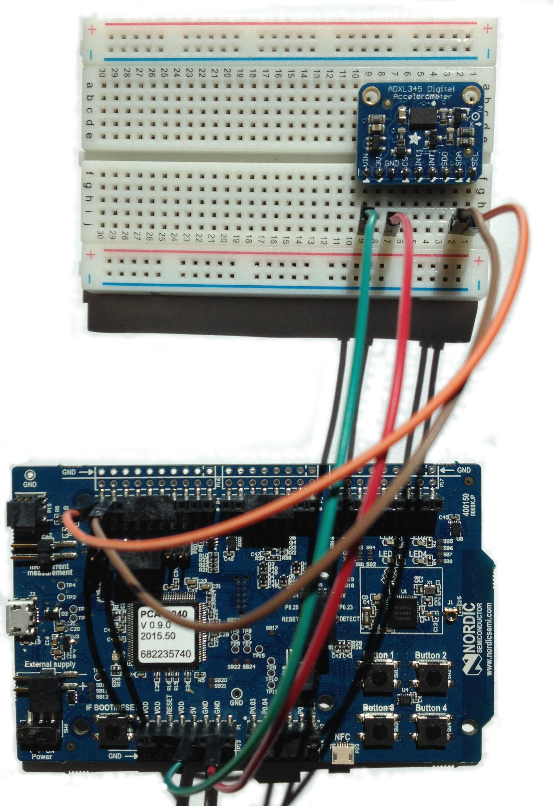
\includegraphics[width=0.62\textwidth]{connectionADXL-nrf5.png}    
    \caption{Connected nRF52 -- ADXL345}
    \label{fig:nrf-adxl345}
\end{figure}

\newpage

\noindent \gls{nRF52} supports both \gls{i2c} and \gls{spi} serial computer buses. \gls{i2c} was chosen in this case, because it is fast enough, flexible and simple to set up with use of few cables. As seen in table \ref{nRF52ADXL345connection} and in figure \ref{fig:nrf-adxl345}, this interface only requires four cables, for power, ground, data and clock. This gives a bandwidth of 1 bit and a maximum bitrate of 5 Mbit/s \cite{semiconductors2000i2c}. The is approximately the same as the assumed max rate capable from the \gls{nRF52}. 

\noindent After the physical connection was complete, it was possible to start the process of initializing the \gls{ADXL345}. Acceleration values can only be read from this sensor if this has been correctly initialized at compile time. In order to do so, code to write to and read from the registers had to be added. To establish this communication, another example from Nordic Semiconductor was used as a starting point, named \textit{TWI master with TWI slave}. By using specific methods from this example and writing to the right accelerometer registers in the right order \cite{devices2009digital}, it was possible to configure the accelerometer as wanted. The detailed description of the programming code used to do this can be seen in appendix \ref{chp:appendixc}. 

\noindent It turned out to be difficult and very time consuming to configure the \gls{ADXL345} to work as expected with the \gls{nRF52}. In short, registers for \textit{data format control, initial power saving, interrupt enable control} and \textit{the offset of each axis} has to be written to in that order. After this, the acceleration value from the different axes can be read. It was then possible to read from the registers containing current acceleration values using the following code: 

\begin{lstlisting}[language=C]

static uint16_t read_reg(uint8_t register_address, uint8_t data_returnValue) 
{
	uint16_t rd;
	ret_code_t ret;
	uint8_t buff[2];
    uint8_t addr8 = (uint8_t)register_address;
    
    ret = nrf_drv_twi_tx(&m_twi_master, ADXL345_SLAVE_ADDRESS, &addr8, 1, true);
    if(NRF_SUCCESS != ret)
    {
        break;
    }
    ret = nrf_drv_twi_rx(&m_twi_master, ADXL345_SLAVE_ADDRESS, buff, 2, false);
	rd = (uint16_t)(buff[0] | (buff[1] << 8));
    
    return rd;	
}

\end{lstlisting}


\noindent In the solution proposed in this thesis the acceleration values are being read as often as possible, limited by the processing power of the \gls{nRF52} and the \gls{i2c} connection. Furthermore, the read value is being stored in a simple dynamic char array in the \gls{nRF52} before being sent and reset when the \gls{ble} channel is ready. The highest obtained measurement frequency in this system was 11 times per main loop, and 150 within this, resulting in 1650 measurements every second. The \gls{ADXL345} updates its acceleration value when instructed by the master, and the default setting is to follow the oscillator \textit{tick} of the \gls{nRF52}. This gives an update approximately every second. The result was that even though the register was being read as often as possible, the same value was read up to 1650 times before it was updated. 



\noindent To solve this problem the default setting of updating the register when told by the oscillator needed to be changed. This turned out to be very time consuming and hard to solve in a proper way, both because of problems with initializing the accelerometer correctly and making the \gls{nRF52} read and store the values fast enough to get proper data. The ideal solution would be to read at least 1000 values every second, to get a good starting point before analysing values. At this point it was not possible to get enough real data to be used in data analysis at another point in the system. In order not to loose too much time on hardware problems, it was decided to focus more on analysing the data sent over the network communication with random generated data. 

%\noindent It would have been possible to use these values to test the network, even though the same value were read several times in a row. However, the accelerometer did never give a fixed number of measured values, and all the measured values could be from 0 to 5 digits long. Since the main focus of this thesis is to understand how data travels through the network, it was decided to not focus further on getting real data due to hardware problems. It would be preferable for the network measurements to use predictable data of fixed length, to get directly comparable results. To test the system with real data will therefore be discussed in the future work section, in chapter \ref{chp:results}. Since the network connection between the \gls{nRF52} and \gls{Raspberry Pi} was already stable, it was easy to generate random values of fixed length to send on the \gls{nRF52}, and do measurements to calculate the optimal throughput between these two. 

\noindent The next chapter will describe the data analysis of the data sent through this network in detail, and how to optimize the percentage of usable data being transported.  

\newpage

\section{Discussion}

\noindent Now the full system shown in figure \ref{fig:systemArchitectureThisSystem} has been connected. Due to problems explained in the previous section, the rest of the thesis will focus mainly on the link between the \gls{nRF52} and the \gls{Raspberry Pi}, with the option of using extra computational power from the stationary computer or a web service if necessary. The central point of discussion at this point is how to process and analyse data in the system. The main options to consider in all the different devices concerning how much computation to do in this link are the following: 

\begin{itemize}
  \item Useful raw data: All data arrives as useful data, and can be posted directly to a web page or a server for storage
  \item No computation: Forward all data directly to a computer with more computational power
  \item Some computation: Analyse the data to find data that is not relevant to filter out
  \item Full computation: Do a full analysis of the data. The results can then be posted directly to a server or displayed on a web page. 
\end{itemize}

\todo{Forenkle. Se Franks kommentarer.}
\noindent The most relevant option of these four depends on the data, and on how much computational power is needed. It is possible to run the Raspberry Pi from a power bank, but this has not been tested in this project. When set up without a battery as power source, the Pi is the first node that could possibly do computations without having to take power limitations as a major concern. The main limitation is therefore computational power, while the main limitation may be battery power on the nRF52. It therefore makes sense to do some easy computation on this device. For instance, if this network is being used to measure vibrations, it is reasonable to assume that measurements more frequent than once every 100 \textit{ms} is needed. Any less frequent than this and vibrations could be missed, especially if it is periodical. It would then be perfectly reasonable to assume that the Pi could go through these values, and calculate whether or not the current acceleration value has breached a given threshold. This result can then be displayed directly on a web page or a connected monitor from the Pi. If however the system is to calculate \textit{patterns} in the acceleration values, several values needs to be compared together. The need of complex algorithms to find these patterns is expected, before the results can be displayed. In this case it is reasonable to assume that the Pi would need additional computational power. The Pi can then be set up as a forwarding device, that forward data directly to a computer with more computational power. 



%\subsection{Connection Challenges} %\todo{Move to appendix, or change? Typ: Planned to this, that didnt work because of this, we did this instead}

%\noindent Following instructions from a representative from Nordic Semiconductor, the bt0 interface was set up using the recommended \gls{ipv6} prefix: \textit{2001:bt8::1/64} in in the file \textit{/etc/sysctrl.conf}, and after that trying to connect and test the connected devices using addresses on the form: 

%\begin{verbatim}
%ping6 2001:bt8::0211:22FF:FE33:4455
%\end{verbatim}

%\noindent This turned out not to work on the \gls{ipv6} network used on \gls{ntnu}, where the standard prefix is \textit{2001::1/64}, without the \textit{db8}. Both solutions should however work in other \gls{ipv6} networks. 



